\documentclass[border=2pt]{standalone}
\usepackage{amsmath}
\usepackage{xcolor}
\usepackage{tikz}
\usetikzlibrary{arrows.meta,positioning}
\begin{document}
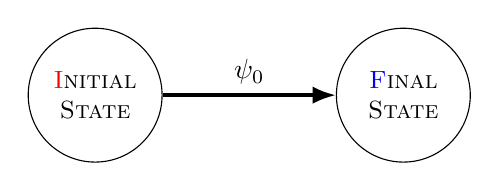
\begin{tikzpicture}[>=Latex]
  \node[
    draw,
    circle,
    minimum size=1.7cm,
    align=center,
    font=\small\scshape
  ] (initial) {\textcolor{red}{I}nitial\\State};
  \node[
    draw,
    circle,
    minimum size=1.7cm,
    align=center,
    font=\small\scshape,
    right=2.2cm of initial
  ] (final) {\textcolor{blue}{F}inal\\State};
  \draw[->,very thick] (initial) -- node[above] {$\psi_0$} (final);
\end{tikzpicture}
\end{document}
